\section{Maciej Trzaskacz}

Wyrażenie matematyczne: \[\sqrt{a^2+b^2}=c\]


Zdjecie psa (Rysunek~\ref{fig:pies})
\begin{figure}[htbp]
    \centering
    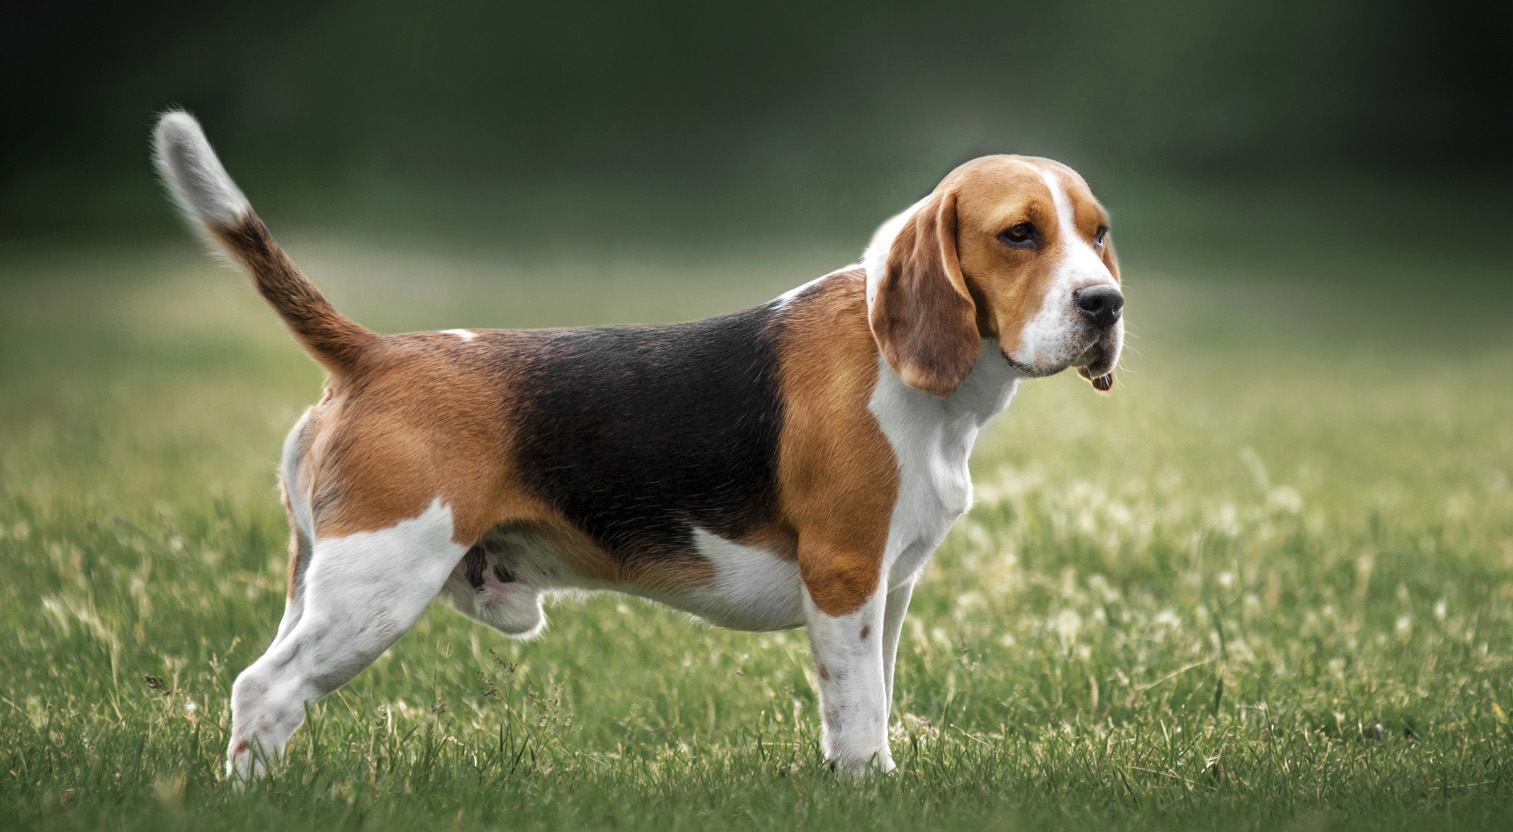
\includegraphics[width=0.5\textwidth]{pictures/pies.jpg}
    \caption{Pies rasy beagle}
    \label{fig:pies}
\end{figure}
    
Tabela~\ref{tab:przykladowa_tabela}
\begin{table}[htbp]
\centering
\begin{tabular}{|l|l|l|l|l|}
\hline
\textbf{}  & \textbf{A} & \textbf{B} & \textbf{C} & \textbf{D} \\ \hline
\textbf{1} & A1         & B1         & C1         & D1         \\ \hline
\textbf{2} & A2         & B2         & C2         & D2         \\ \hline
\textbf{3} & A3         & B3         & C3         & D3         \\ \hline
\end{tabular}
\caption{Przykładowa tabela}
\label{tab:przykladowa_tabela}
\end{table}

    Lista numerowana:
    \begin{enumerate}
        \item item 1
        \item item 2
        \item item 3
    \end{enumerate}
    
    Lista nienumerowana:
    \begin{itemize}
        \item item
        \item[->] other item
        \item[*] another item
    \end{itemize}

    \textbf{Lorem ipsum dolor sit amet}, consectetur adipiscing elit. Maecenas mollis facilisis nisl, auctor rutrum neque ullamcorper et. Mauris varius semper orci \textit{porta feugiat}.
    
    Vestibulum mattis lectus condimentum, volutpat nibh mattis, mattis leo. Maecenas semper \underline{turpis quis turpis gravida} rhoncus. Sed finibus, orci sit amet tincidunt ultrices, nulla lorem tincidunt ipsum, in tincidunt eros nisl sit \textbf{\textit{\underline{amet libero}}}.